\section{Consequences of the \MLIR Design}

The \MLIR design facilitates the modeling of new language and compilation abstractions while reusing existing, generic ones as well as their associated compilation methods. Effectively,
the solution to many problems is to ``add new ops, new types'', possibly collected into
``a new dialect''.  This is a significant design shift for compiler engineering.
It produces new opportunities, challenges, and insights.  This section
explores a few of them.

%====================================
\subsection{Reusable compiler passes}
\label{sec:reusable_passes}
%====================================

The ability to represent multiple levels of abstraction in one IR creates the
natural desire to write passes that work across multiple levels of abstraction. A
common question about \MLIR is ``how do you write a compiler pass when you have
openly extensible operations and type system?'' While it is always possible
for a compiler pass to treat unknown constructs in a conservatively correct
way, our goal is to produce high performance code, so we need to do
useful things in common cases. We have found four major approaches:

%-------------------------------------------
\paragraph{Fundamental operation traits}
%-------------------------------------------

Some ``bread and butter'' compiler passes like Dead Code Elimination and Common
Subexpression Elimination rely on very simple properties (like ``has no
side effect'' or ``is commutative'') that we define as Op traits.  The definition
of an operation in ODS allows the author of the operation to specify these
traits, and passes can uses this information to remain applicable
across many different abstraction domains.

\MLIR is extensible enough that it has a few structural properties, including
information about whether an operation is known to be a control flow terminator,
whether an operation containing a region is known to be isolated-from-above, etc.
These allow generic modeling and
processing of functions, closures, modules, and other code structures.

%-----------------------------------------
\paragraph{Privileged operation hooks}
%-----------------------------------------

While certain traits can be modeled with a single bit, others need \Cpp code to
provide an implementation---constant folding logic for example. \MLIR has first
class support for certain hooks applicable to a large number of passes. These
hooks can either be implemented on a per-operation basis, or in
the Dialect object itself. The later approach is
convenient for things like constant folding of TensorFlow ops, where delegation
to existing logic is straightforward.

While constant folding is very important functionality, a more interesting hook
is \lstinline|getCanonicalizationPatterns|, which allows one to specify folding
patterns that apply to an operation.  This enables open extensibility of important
algebraic simplifications (e.g. $x-x \rightarrow 0$, $\min(x,y,y) \rightarrow \min(x,y)$ etc.) and powers
a common ``Canonicalization'' pass that can now be applied to all dialects.  This
allows this single extensible system to subsume things like
``InstCombine'', ``DAGCombine'', ``PeepholeOptimizer'', ``SILCombine'', and
other special purpose passes seen in the LLVM ecosystem (and other
compilers), which are a well-known maintenance and complexity burden.

%--------------------------------------
\paragraph{Optimization interfaces}\label{sec:interfaces}
%--------------------------------------

A primary goal of \MLIR is to allow open extensibility---not just in terms of
operations and types, but also in terms of transformations.  While canonicalization
and constant folding are critical operations, there are a number of standard
transformations that need to be parameterized in certain ways---e.g., to describe
transformation specific properties, to implement cost models, etc.

The solution is a subsystem known as ``Optimization Interfaces''. Consider the
\MLIR inlining pass: we would like the inliner to work on TensorFlow graphs,
Flang functions, closures in a functional language etc.---but the inliner does
not know what call sites or even the callees are! The core characteristics that
an inliner needs to know are:

\begin{itemize}
\item whether it is valid to inline an operation into a given region;
\item how to handle terminator operations that ended up in the middle of a block
after inlining.
\end{itemize}


\begin{figure}[h]
  \centering
  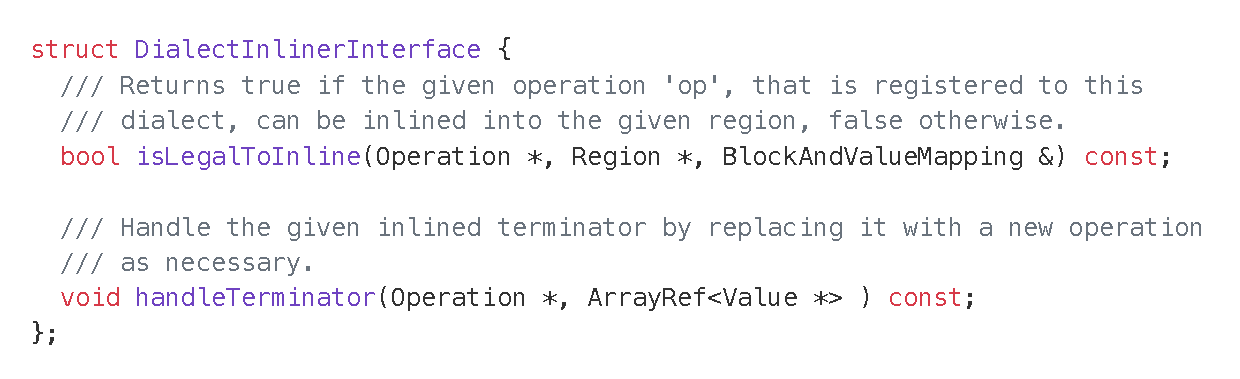
\includegraphics[width=.85\textwidth]{img/dialect_interface.pdf}
	%\begin{tabular}{c}
	%\begin{lstlisting}[language=c++]
	%struct DialectInlinerInterface {
	%  /// Returns true if the given operation 'op', that is registered to this
	%  /// dialect, can be inlined into the given region, false otherwise.
	%  bool isLegalToInline(Operation *, Region *, BlockAndValueMapping &) const;
	%
	%  /// Handle the given inlined terminator by replacing it with a new operation
	%  /// as necessary.
	%  void handleTerminator(Operation *, ArrayRef<Value *> ) const;
	%};
	%\end{lstlisting}
% \end{tabular}
\caption{Dialect interface to query legality of inlining.}\label{fig:inlining}
\end{figure}

In order to know these properties, the Inliner pass defines the interface
in~\figref{inlining}. Individual operations and dialects may register their
implementation of this interface with \MLIR to benefit from the generic inliner
pass. If an operation or dialect fails to provide an interface then the
corresponding optimization pass will treat the operation conservatively. This
design allows the implementer of a dialect to get up and
running quickly, but derive more value out of the system by putting more
implementation effort into interfaces likes these over time.

Optimization interfaces also provide modularity benefit for the core compiler, because the
dialect specific logic is implemented within the dialects themselves, instead of
inside the core transformations.

%-------------------------------------
\paragraph{Dialect specific passes}
%-------------------------------------

Finally, it is valid and useful to define passes that are specific to particular
dialects, which can be driven by full semantics of operations in the dialect(s) they are
designed for.  These passes are just as useful in the \MLIR system as they
are in other compiler systems.  For example, code generators that want to do
custom scheduling of machine instructions based on particular machine constraints
or other tricks that do not fit into a broader framework. This is a simple and
useful starting point for new transformations, where generalization isn't required.

%====================================
\subsection{Mixing dialects together}
%====================================

One of the most profound (but also most difficult to grok) aspects of \MLIR
is that it allows and encourages mixing operations from different dialects
together into a single program.  While certain cases of this are reasonably
easy to understand (e.g. holding host and accelerator computation in the same
module) the most interesting cases occur when dialects are directly mixed---
because this enables an entire class of reuse that we have not seen in other
systems.

Consider the affine dialect described in \secref{affine}. The definition
of affine control flow and affine mappings are independent of the semantics of
the operations that are contained in affine regions.  In our case, we combine
the affine dialect with the ``standard'' dialect that represents simple arithmetic
in a target independent form like LLVM IR, with multiple target-specific machine
instruction dialects for internal accelerators. Others have combined it with
abstractions from other problem domains.

The ability to reuse generic polyhedral transformations (using Op interfaces to
get semantics of operations in specific transformations) is a powerful (and
exciting to us) way of factoring compiler infrastructure. Another
example is that an OpenMP dialect could be used and reused across a wide variety
of source-language IRs.

%============================
\subsection{Interoperability}
%============================

Our work involves interoperation with a large number of existing systems, e.g.,
machine learning graphs encoded as protocol buffers, compiler IRs including
LLVM IR, proprietary instruction sets, etc.  Often the representation has a
number of suboptimal or unfortunate decisions that made sense in the context of
an existing system, but capabilities of \MLIR enable a more expressive
representation. Because importers and exporters are notoriously
difficult to test (often the test cases are binary formats), we want to make
sure their complexity is minimized.

The solution is to define a dialect that corresponds to the foreign system as
directly as possible---allowing round tripping to-and-from that format in a simple
and predictable way. Once the IR is imported into \MLIR form, it can be raised
and lowered to a more convenient IR using all of the \MLIR infrastructure for doing
these transformations, and allows those transformations to be tested similarly
to all the other \MLIR passes are.

There are numerous examples of such dialects, including: a) the LLVM dialect---which
maps LLVM IR into \MLIR, b) the representation of TensorFlow graphs---which
is raised to ease analysis and transformations related to ``switch and merge''
nodes in TensorFlow, and c) functional-style control flow operators---``functional
while'' and ``functional if'' are common in machine learning graphs, in which it is
more convenient to work with their bodies as regions instead of out-of-line
functions.

This approach has worked well for us, and the \MLIR tooling has also been useful
to write tests for these foreign binary file formats.

%======================================================
\subsection{Unopinionated design provides new challenges}
%======================================================

While \MLIR allows one to define almost arbitrary abstractions, it provides very
little guidance on what \emph{should} be done: what works better or worse in
practice? We now have some experience with a number of engineers and researchers
applying the techniques and technologies to new problem domains, and have
realized that the ``art'' of compiler IR design and abstraction design is not
well understood in the compiler and languages field---many people work within
the constraints of established systems, but relatively few have had the
opportunity define the abstractions themselves.

This is a challenge, but is also another set of opportunities for future research.
The broader \MLIR community is building a significant amount of expertise with these
abstraction design trade-offs, and we expect this to be a fertile area of study over
time.

%===========================
\subsection{Looking forward}
%===========================

The design of \MLIR is different enough from other compiler infrastructures that
we are still learning---even after building and applying it to many different
systems. We believe that there is still a lot to discover, and several more
years of research will be required until the design points are all fully
understood and best practices are established. For example, the rise of
out-of-tree dialects, increasing number of source language frontends using
\MLIR, possible application to Abstract Syntax Trees, and applications to
structured data (like JSON, protocol buffers, etc) which are still very early
and are likely to uncover interesting new challenges and opportunities.
